\documentclass[tikz, border=12pt]{standalone}
\usepackage[scaled=0.95]{helvet}
\renewcommand{\familydefault}{\sfdefault}

\definecolor{espressocolor}{RGB}{170, 85, 20}
\definecolor{milkcolor}{RGB}{40, 110, 190}
\definecolor{coldcolor}{RGB}{20, 150, 130}

\begin{document}
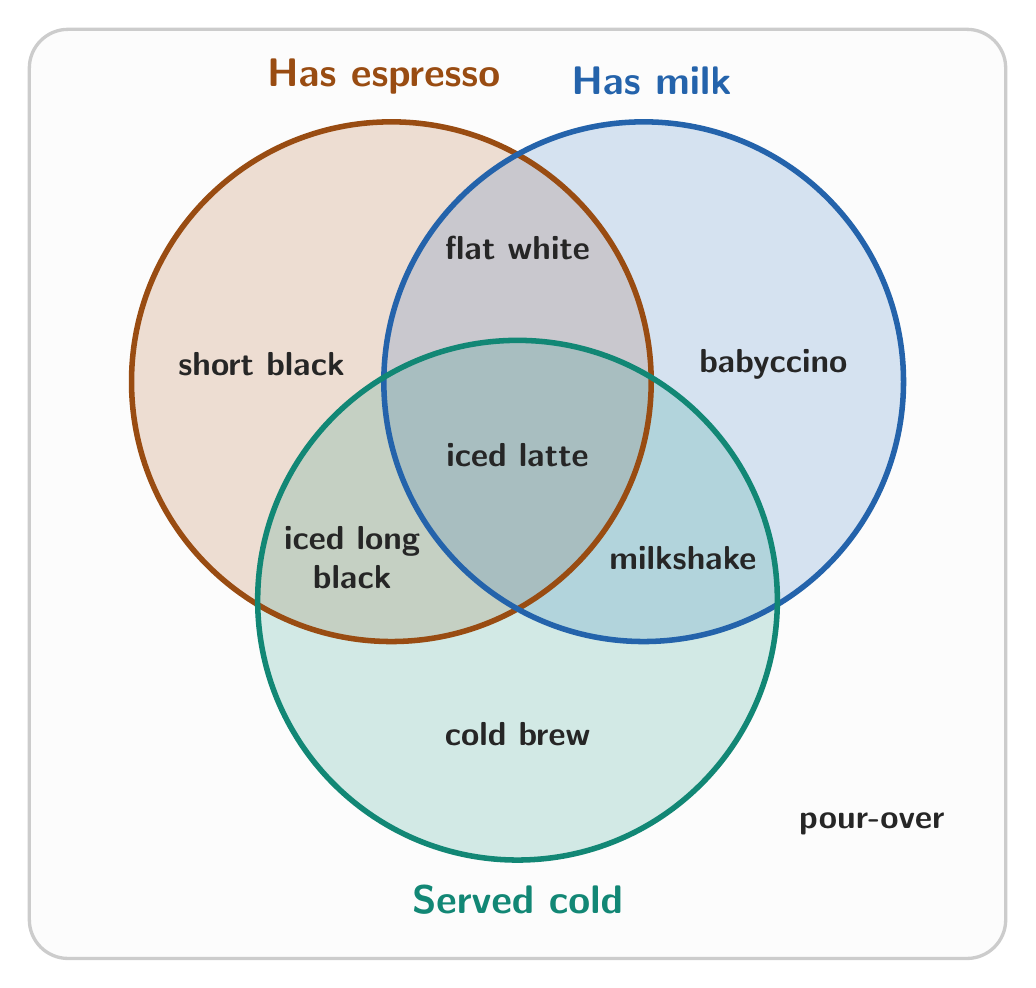
\begin{tikzpicture}[>=latex]

  % Bounding box representing the universe of drinks
  \draw[rounded corners=14pt, line width=1.2pt, gray!40, fill=gray!2] (-6.2, -6.4) rectangle (6.2, 5.4);

  % Circle coordinates: radius 3.3cm, centers at distance 1.85cm at 150°, 30°, 270°
  \coordinate (A) at (150:1.85);
  \coordinate (B) at (30:1.85);
  \coordinate (C) at (270:1.85);
  \def\rad{3.3cm}

  % Translucent fills
  \begin{scope}[fill opacity=0.18]
    \fill[espressocolor] (A) circle (\rad);
    \fill[milkcolor] (B) circle (\rad);
    \fill[coldcolor] (C) circle (\rad);
  \end{scope}

  % Circle borders
  \draw[espressocolor!90!black, line width=2pt] (A) circle (\rad);
  \draw[milkcolor!90!black, line width=2pt] (B) circle (\rad);
  \draw[coldcolor!90!black, line width=2pt] (C) circle (\rad);

  % Set labels
  \node[font=\bfseries\Large, text=espressocolor!90!black, anchor=south] at (-1.7, 4.45) {Has espresso};
  \node[font=\bfseries\Large, text=milkcolor!90!black, anchor=south] at (1.7, 4.45) {Has milk};
  \node[font=\bfseries\Large, text=coldcolor!90!black, anchor=north] at (0, -5.35) {Served cold};

  % --- Drinks ---
  % 1. Has espresso only
  \node[font=\bfseries\large, text=black!85, align=center] at (-3.25, 1.15) {short black};

  % 2. Has milk only
  \node[font=\bfseries\large, text=black!85, align=center] at (3.25, 1.15) {babyccino};

  % 3. Served cold only
  \node[font=\bfseries\large, text=black!85, align=center] at (0, -3.55) {cold brew};

  % 4. Has espresso + Has milk (not cold)
  \node[font=\bfseries\large, text=black!85, align=center] at (0, 2.62) {flat white};

  % 5. Has espresso + Served cold (no milk)
  \node[font=\bfseries\large, text=black!85, align=center] at (-2.10, -1.31) {iced long\\black};

  % 6. Has milk + Served cold (no espresso)
  \node[font=\bfseries\large, text=black!85, align=center] at (2.10, -1.31) {milkshake};

  % 7. All three: Has espresso + Has milk + Served cold
  \node[font=\bfseries\large, text=black!85, align=center] at (0, 0) {iced latte};

  % 8. Outside all three sets
  \node[font=\bfseries\large, text=black!85, align=center] at (4.5, -4.7) {pour-over};

\end{tikzpicture}
\end{document}
